\documentclass[11pt]{scrartcl}
\usepackage{tikz}
\usetikzlibrary{calc}
\tikzset{%
    add/.style args={#1 and #2}{
        to path={%
 ($(\tikztostart)!-#1!(\tikztotarget)$)--($(\tikztotarget)!-#2!(\tikztostart)$)%
  \tikztonodes},add/.default={.2 and .2}}
}  


\tikzset{%
  mark coordinate/.style={inner sep=0pt,outer sep=0pt,minimum size=2pt,
    fill=black,circle}%
}

\newcommand\pgfmathsinandcos[3]{%
  \pgfmathsetmacro#1{sin(#3)}%
  \pgfmathsetmacro#2{cos(#3)}%
}
\newcommand\LongitudePlane[2][current plane]{%
  \pgfmathsinandcos\sinEl\cosEl{\Elevation} % elevation
  \pgfmathsinandcos\sint\cost{#2} % azimuth
  \tikzset{#1/.estyle={cm={\cost,\sint*\sinEl,0,\cosEl,(0,0)}}}
}
\newcommand\LatitudePlane[2][current plane]{%
  \pgfmathsinandcos\sinEl\cosEl{\Elevation} % elevation
  \pgfmathsinandcos\sint\cost{#2} % latitude
  \pgfmathsetmacro\ydelta{\cosEl*\sint}
  \tikzset{#1/.estyle={cm={\cost,0,0,\cost*\sinEl,(0,\ydelta)}}} %
}
\newcommand\DrawLongitudeCircle[1]{
  \LongitudePlane{#1}
  \tikzset{current plane/.prefix style={scale=\R}}
  \pgfmathsetmacro\angVis{atan(sin(#1)*cos(\Elevation)/sin(\Elevation))} %
  \draw[current plane,thin,black]  (\angVis:1)     arc (\angVis:\angVis+180:1);
  \draw[current plane,thin,dashed] (\angVis-180:1) arc (\angVis-180:\angVis:1);
}%

\newcommand\DrawLatitudeCircle[1]{
  \LatitudePlane{#1}
  \tikzset{current plane/.prefix style={scale=\R}}
  \pgfmathsetmacro\sinVis{sin(#1)/cos(#1)*sin(\Elevation)/cos(\Elevation)}
  \pgfmathsetmacro\angVis{asin(min(1,max(\sinVis,-1)))}
  
 \draw[current plane,thick, line width=1pt, ] (\angVis:1) arc (\angVis:-\angVis-180:1);

  \draw[current plane,line width=1pt, opacity=0.2] (180-\angVis:1) arc (180-\angVis:\angVis:1);
}%





\begin{document}
  \null\vfill
\begin{center}
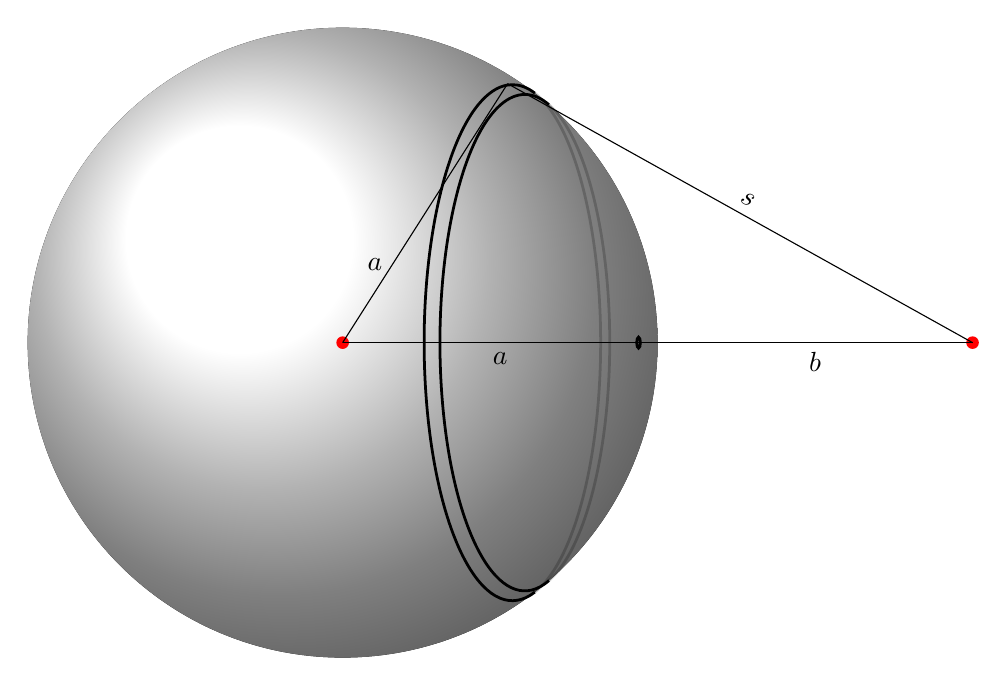
\begin{tikzpicture}[rotate=-90]
    \def\R{4} % sphere radius
    \def\Elevation{20} % elevation angle
    \fill[ball color=white!10] (0,0) circle (\R); % 3D lighting effect
    \foreach \i in {35,38,89} {\DrawLatitudeCircle{\i}}
    \fill[red] (0,0) circle (0.08);
    \fill[red] (0,8) circle (0.08);
    \draw (0,\R) -- node[below] {$b$} (0,8) coordinate (P);
    \draw (0,0) -- node[below] {$a$} (0,\R);
    \draw (0,0) -- node[pos=0.3,anchor = east] {$a$} ({180-32.5}:\R-0.1) coordinate (B);
    \draw (B) -- node [above, sloped, rotate=-90] {$s$}(P);
\end{tikzpicture}   
\end{center}


\end{document}  